\chapter{Internship description}\label{cap:internship-desc}
\intro{This chapter will describe the internship project, the requirements and the goals.}
\section{Initial analysis}
Given the idea of the project, the first step was to analyze the requirements for get a GAN model that was able to do the job.
Some questions were made to understand what we want to achieve and how to do it.
\begin{itemize}
    \item\textbf{What kind of images the model should generate?}
    \item\textbf{What kind of images the model should receive as input?}
    \item\textbf{What kind of network should be used?}
    \item\textbf{What kind of features should be extracted from the images?}
    \item\textbf{What kind of dataset should be used?}
\end{itemize}
From the previous questions, was possible to define Requirements, Goals and a road-map for the project.\\
\section{Requirements \& Goals}
\subsection{Requirements}
\begin{itemize}
    \item \textbf{Requirement 1}: The dataset should be composed by high quality images;
    \item \textbf{Requirement 2}: The model should be able to generate images from a given input, like a sketch;
    \item \textbf{Requirement 3}: The model should be able to generate images with a good quality, comparable with the real images;
    \item \textbf{Requirement 4}: The generated images should be previewed in real time;
\end{itemize}
\subsection{Goals}
\begin{itemize}
    \item \textbf{Goal 1}: Obtain a dataset of images with a good quality and variety;
    \item \textbf{Goal 2}: Obtain a model that is able to generate images from a sketch;
    \item \textbf{Goal 3}: Obtain a desktop application that is able to generate images in real time and preview them;
\end{itemize}
\section{Planning}
Initially, the project was planned using a story map~\ref*{label:story-map} to define the main features of the project and the main steps to achieve them.
\begin{figure}[H]
    \centering
    \includegraphics[width=1\textwidth]{images/story-map.jpg}
    \caption{Story map}\label{label:story-map}
\end{figure}
\subsection{Road-map}
After an Initial analysis of the story map, was possible to define a road-map for the project based on requirements and goals to achieve in the Internship period.
All the activity has been planned using a specific division of the time in different phases.
\begin{itemize}
    \item \textbf{Train period}: study of the state of the art and the technologies that will be used;
    \item \textbf{First period}: images acquisition;
    \item \textbf{Second period}: dataset increase, images augmentation;
    \item \textbf{Third period}: main feature extraction;
    \item \textbf{Fourth period}: network training;
    \item \textbf{Fifth period}: results analysis and improvement;
\end{itemize}
\begin{landscape}
\begin{ganttchart}[%Specs
    y unit title=0.5cm,
    y unit chart=0.6cm,
    x unit=1.0cm,
    vgrid,hgrid,
    title height=1,
%     title/.style={fill=none},
    title label font=\bfseries\footnotesize,
    bar/.style={fill=blue},
    bar height=0.7,
%   progress label text={},
    group right shift=0,
    group top shift=0.7,
    group height=.3,
    group peaks width={0.2},
    inline]{1}{12}
   %labels
   \gantttitle{Internship Project}{12}\\  % title 1           
   \gantttitle{April}{4}                      % title 3
   \gantttitle{May}{4}
   \gantttitle{June}{4}
   % Setting group if any
   \ganttgroup[inline=false]{Train Period}{2}{3}\\ 
   \ganttbar[progress=100,inline=false]{Technology exploration}{2}{3}\\

   \ganttgroup[inline=false]{First Period}{3}{4}\\ 
   \ganttbar[progress=100,inline=false]{Image acquisition}{3}{4}\\
   \ganttmilestone[inline=false]{Milestone 1}{4} \\

   \ganttgroup[inline=false]{Second Period}{3}{4}\\ 
   \ganttbar[progress=100,inline=false]{Dataset improvements}{3}{4}\\
   \ganttmilestone[inline=false]{Milestone 2}{4} \\

   \ganttgroup[inline=false]{Third Period}{4}{5}\\ 
   \ganttbar[progress=100,inline=false]{Features extraction}{4}{5}\\
   \ganttmilestone[inline=false]{Milestone 3}{5} \\

   \ganttgroup[inline=false]{Fourth Period}{5}{7}\\ 
   \ganttbar[progress=100,inline=false]{Network training}{5}{7}\\
   \ganttmilestone[inline=false]{Milestone 4}{7} \\

   \ganttgroup[inline=false]{Fifth Period}{7}{11}\\ 
   \ganttbar[progress=50,inline=false]{General improvements \& Docs}{7}{11}\\
   \ganttmilestone[inline=false]{Milestone 5}{11} \\
\end{ganttchart}
\end{landscape}
\subsection{Study Period:}
This period was used to study the state of the art and the technologies that will be used during the internship.\\
The main topics were:
\begin{itemize}
    \item \textbf{Machine Learning}: study of the main concepts of machine learning and deep learning;
    \item \textbf{GAN}: study of the main concepts of GAN and how they work;
    \item \textbf{GAN applications}: study of the main applications of GAN and how they are used;
    \item \textbf{GAN architectures}: study of the main GAN architectures and how they are used;
    \item \textbf{GAN training}: study of the main techniques used to train a GAN;\@
    \item \textbf{GAN evaluation}: study of the main techniques used to evaluate a GAN;\@
    \item \textbf{GAN improvements}: study of the main techniques used to improve a GAN;\@
    \item \textbf{GAN applications}: study of the main applications of GAN and how they are used;
\end{itemize}
\subsection{Train Period:}
During this was the acquisition of the images.
Every Breton machine has been equipped with a camera and a computer with a software that allows to acquire images from the camera.
This camera take a picture of each worked slab and send it to the database.
\subsubsection{Problems:}
The main problem in this phase was related to the quality of the images.
The images acquisition of the machine was not meant to be used for a machine learning project, so the quality of the images was not the best.
The images were not all of the same size and the background was not always the same, sometimes they contains reflections of the light or the shadow of the machine.
\subsubsection{Solutions:}
To solve this problems, some precautions were taken.
\begin{itemize}
    \item \textbf{Images background}: the background of the images was removed using a company previously trained \gls{mlg} model that was able to recognize the border of the slab.
                              With this model and OpenCV library it was possible to remove everything that was not the slab from the image.
    \item \textbf{Images defects}: the images contains light reflections and shadows was manually removed from the dataset.
                                   This was possible because the images were not too many.
    \item \textbf{Images size}: the images were resized to a common size, maintaining the aspect ratio.
\end{itemize}
\subsubsection{Milestone:}
At the end of the period the dataset was composed by 7000 images of slabs, with different colors and textures.
The dataset was divided in two parts, one for the training and one for the validation, with a ratio of 70\% and 30\% respectively.
\begin{figure}
    \centering
    \includegraphics[height=6cm]{slabs/intera}
    \caption{Example of a slab}
\end{figure}
\subsection{Second Period:}
During this period the dataset was increased and the images were augmented.
\subsubsection{Augmentation:}
Augmentation is a technique that allows to increase the number of images in a dataset, applying some transformations to the original images.
This technique is useful when the dataset is not big enough to train a network.

The images augmentation technique applied was:
\begin{itemize}
    \item  \textbf{Resize}: each image was resized to a bigger size, from 256$\times$256 to 286$\times$286;
    \item  \textbf{Random Crop}: each image was randomly cropped to a size of 256$\times$256;
    \item  \textbf{Random Flip}: each image was randomly flipped horizontally;
\end{itemize}

For increasing the dataset, each original image was splitted in smaller images of 256$\times$256 pixels.

\subsubsection{Milestone:}

At the end of the period the dataset was composed by 7000 images of slabs, with different colors and textures.


\begin{figure}
    \centering
    \includegraphics[width=.24\textwidth]{slabs/crop/crop_0_0}
    \includegraphics[width=.24\textwidth]{slabs/crop/crop_0_1}
    \\
    \includegraphics[width=.24\textwidth]{slabs/crop/crop_1_0}
    \includegraphics[width=.24\textwidth]{slabs/crop/crop_1_1}
    \caption{Cropped image}\label{fig:foobar}
\end{figure}

\subsection{Third Period:}
This period was dedicated to found the best method to extract the features from the images. (Vein, texture, color, etc.)
Extracting the features from the images is the most important part of the project, because the quality of the features will affect the quality of the network.
So the mask that contains it must be as accurate as possible.

\subsubsection{Vein extraction:}
For the vein extraction, different Python implemented methods were tested.
The methods tested were:
\begin{itemize}
    \item \textbf{Threshold}\footcite{site:opencv-threshold}: this method is based on the Threshold algorithm.
    It consists in the application of a threshold to the image, so that only the pixels with a value higher than the threshold are kept.
    Setting a fixed threshold is not a good idea, because the images have different light conditions.
    So the threshold was calculated using the Otsu's method.
    \item \textbf{Canny Edge Detection}\footcite{site:opencv-canny}: this method is based on the homonym algorithm.
    The Canny algorithm is an edge detection algorithm that uses a multi-stage algorithm to detect a wide range of edges in images.
    The algorithm consists of 5 steps:
    \begin{enumerate}
        \item Noise reduction: the image is smoothed using a Gaussian filter;
        \item Gradient calculation: the intensity gradient of the image is calculated;
        \item Non-maximum suppression: the non-maximum suppression is applied to the gradient image;
        \item Double threshold: two thresholds are used to determine the edges;
        \item Edge tracking by hysteresis: the edges are tracked using the two thresholds.
    \end{enumerate}
    \begin{figure}[H]
        \centering
        \includegraphics[width=.7\textwidth]{slabs/canny/canny}
        \\
        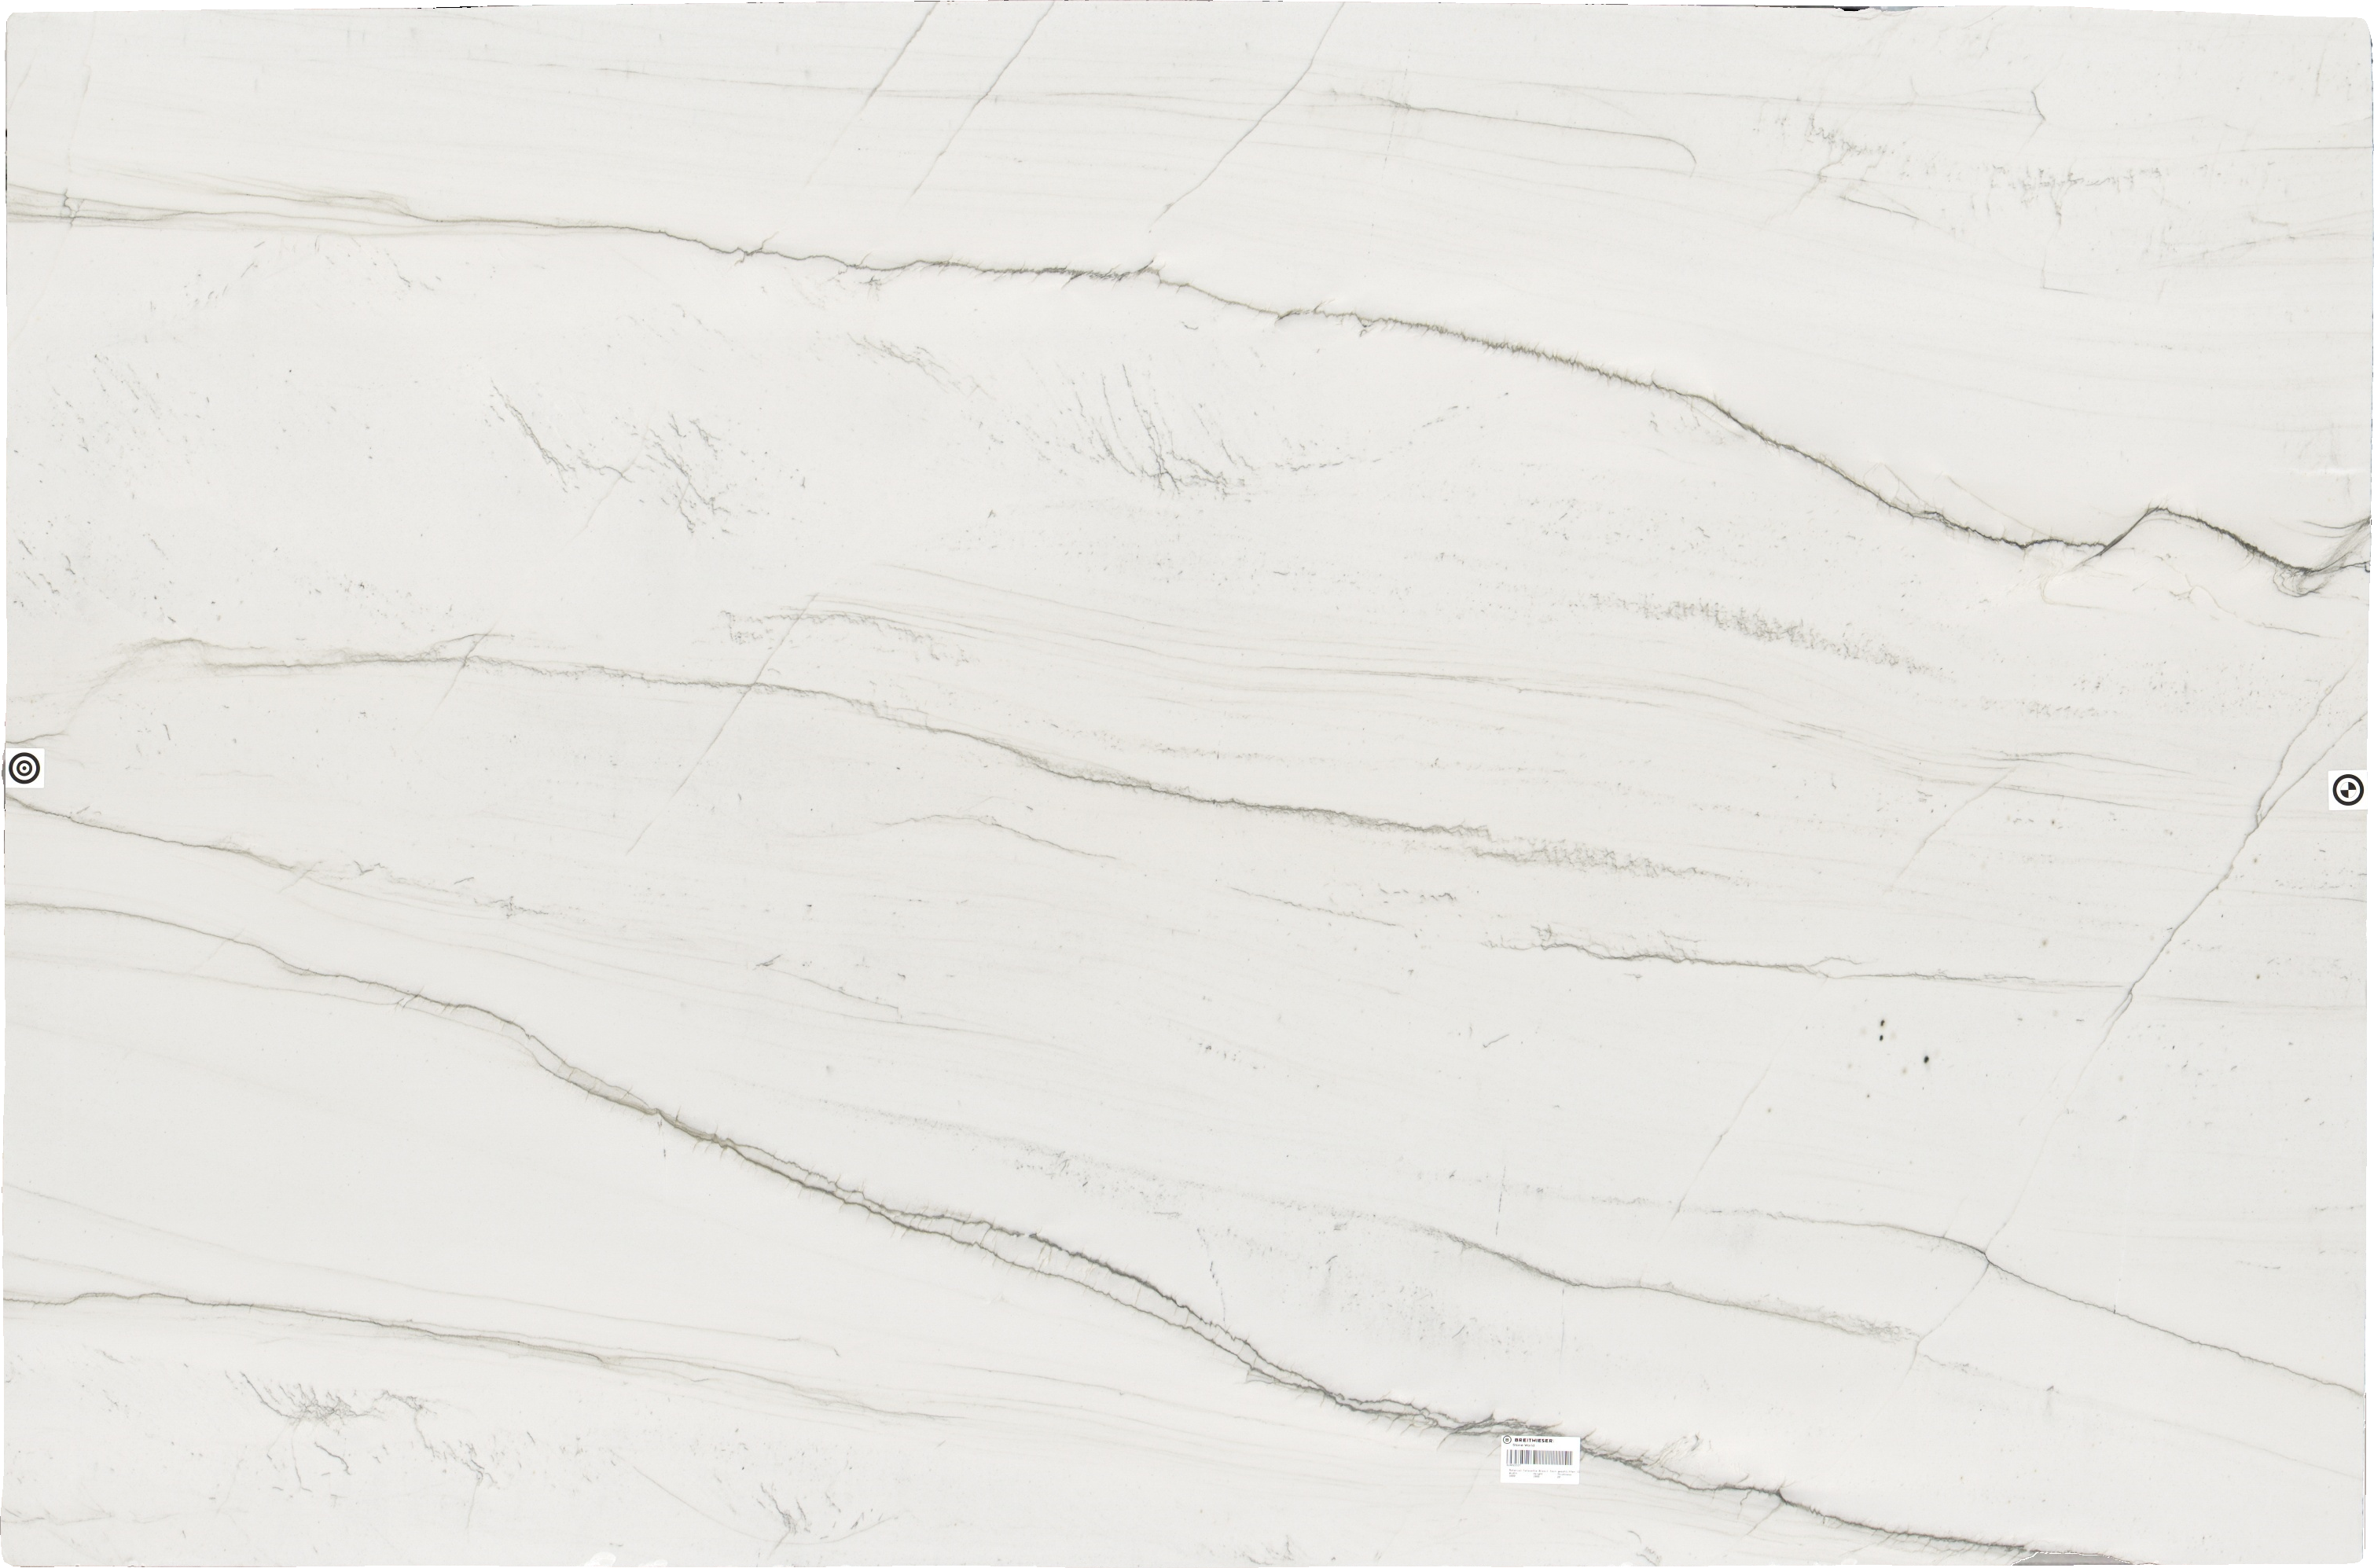
\includegraphics[width=.7\textwidth]{slabs/canny/canny_origin}
        \caption{Canny Edge Detection}\label{fig:canny_compare}
    \end{figure}
    In figure~\ref*{fig:canny_compare} is possible to see the result of the Canny Edge Detection.
    \item \textbf{Meijering \& Contrast filter}\footcite{site:sckit-meijering}: this method uses the Meijering filter to enhance the vein of the image.
    The Meijering filter is a filter that enhances the line-like structures in an image.
    It's based on the Hessian matrix, that is a square matrix containing the second order partial derivatives of a function.
    The Hessian matrix is used to calculate the eigenvalues and eigenvectors of the image.
    The eigenvalues are used to calculate the line-like structures of the image.
    The contrast filter is used to enhance the contrast of the image.
    \begin{figure}[H]
        \centering
        \includegraphics[width=.7\textwidth]{slabs/meijering/meije}
        \\
        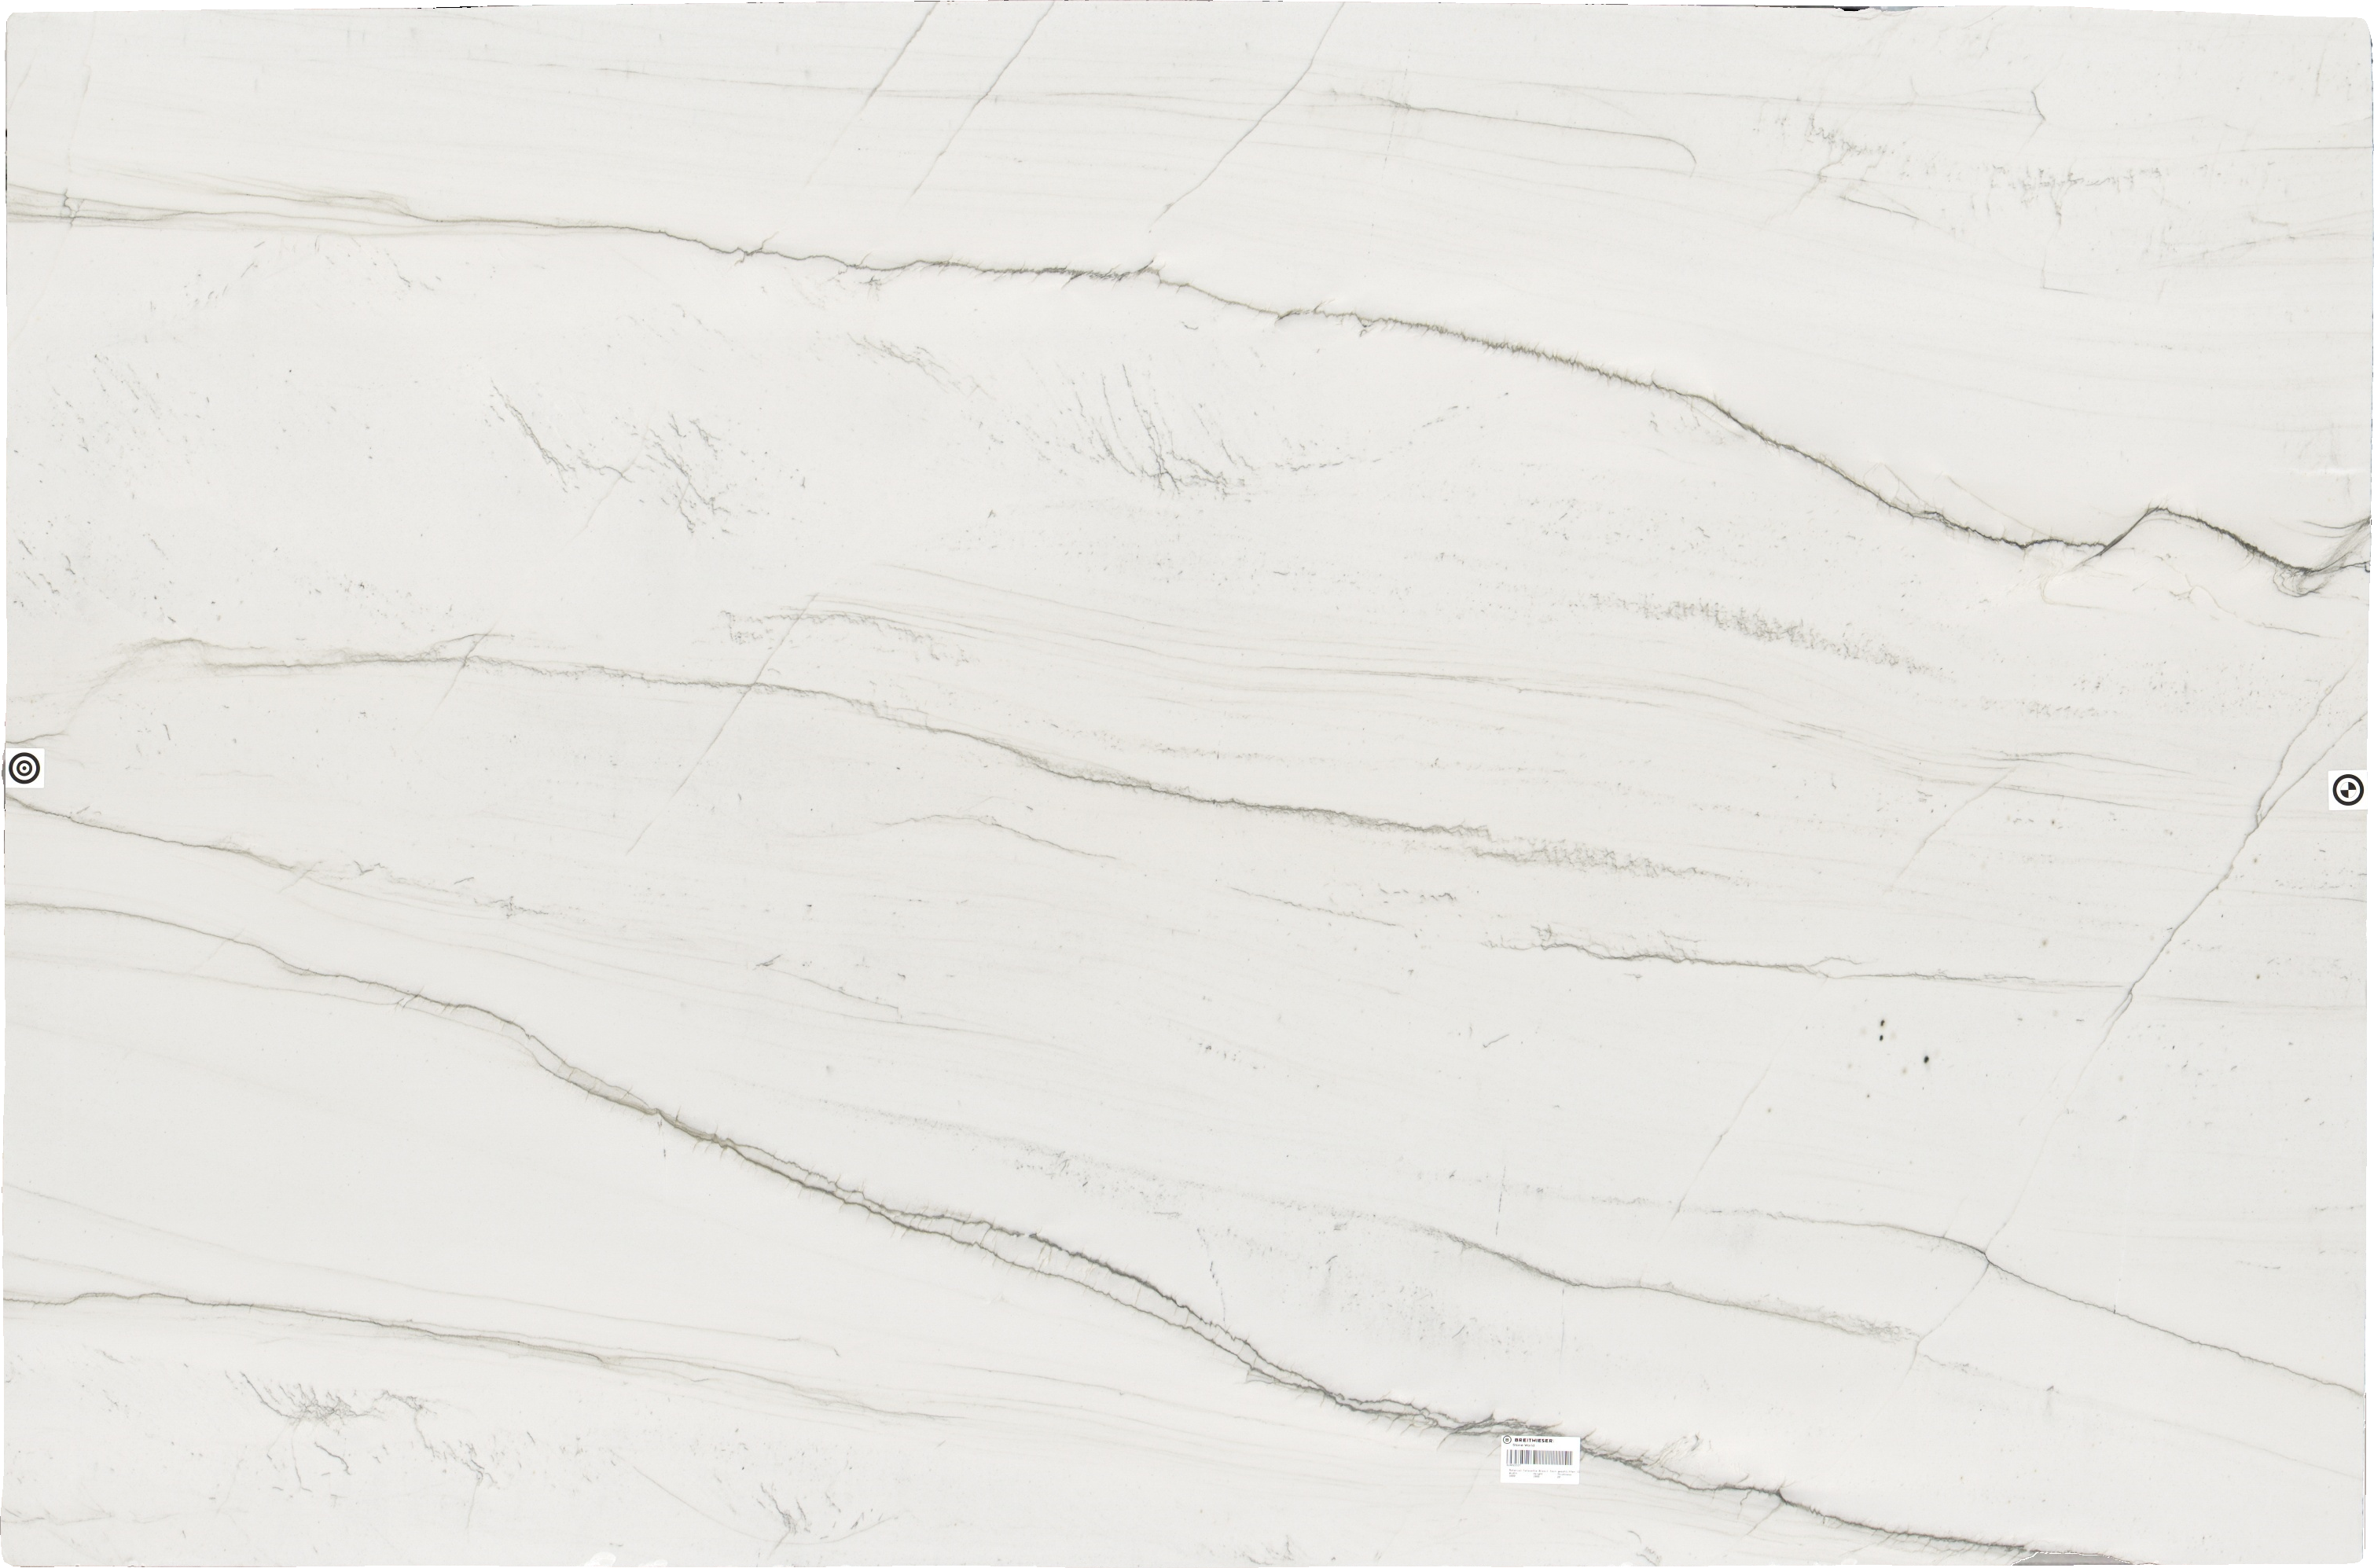
\includegraphics[width=.7\textwidth]{slabs/canny/canny_origin}
        \caption{Meijering \& Contrast filter}\label{fig:meij_compare}
    \end{figure}
    In figure~\ref*{fig:meij_compare} is possible to see the result of the Meijering \& Contrast filter.
    \item \textbf{HED}\footcite{paper:hed}: this method is based on the HED algorithm.
    The HED algorithm is an edge detection algorithm that uses a deep neural network to detect the edges in images.
    The algorithm consists of 3 steps:
    \begin{enumerate}
        \item Pre-trained network: the pre-trained network is used to extract the features from the image;
        \item Multi-scale: the multi-scale algorithm is used to extract the edges from the features;
        \item Edge linking: the edges are linked using the Canny algorithm.
    \end{enumerate}
    \begin{figure}[H]
        \centering
        \includegraphics[width=.7\textwidth]{slabs/hed/hed}
        \\
        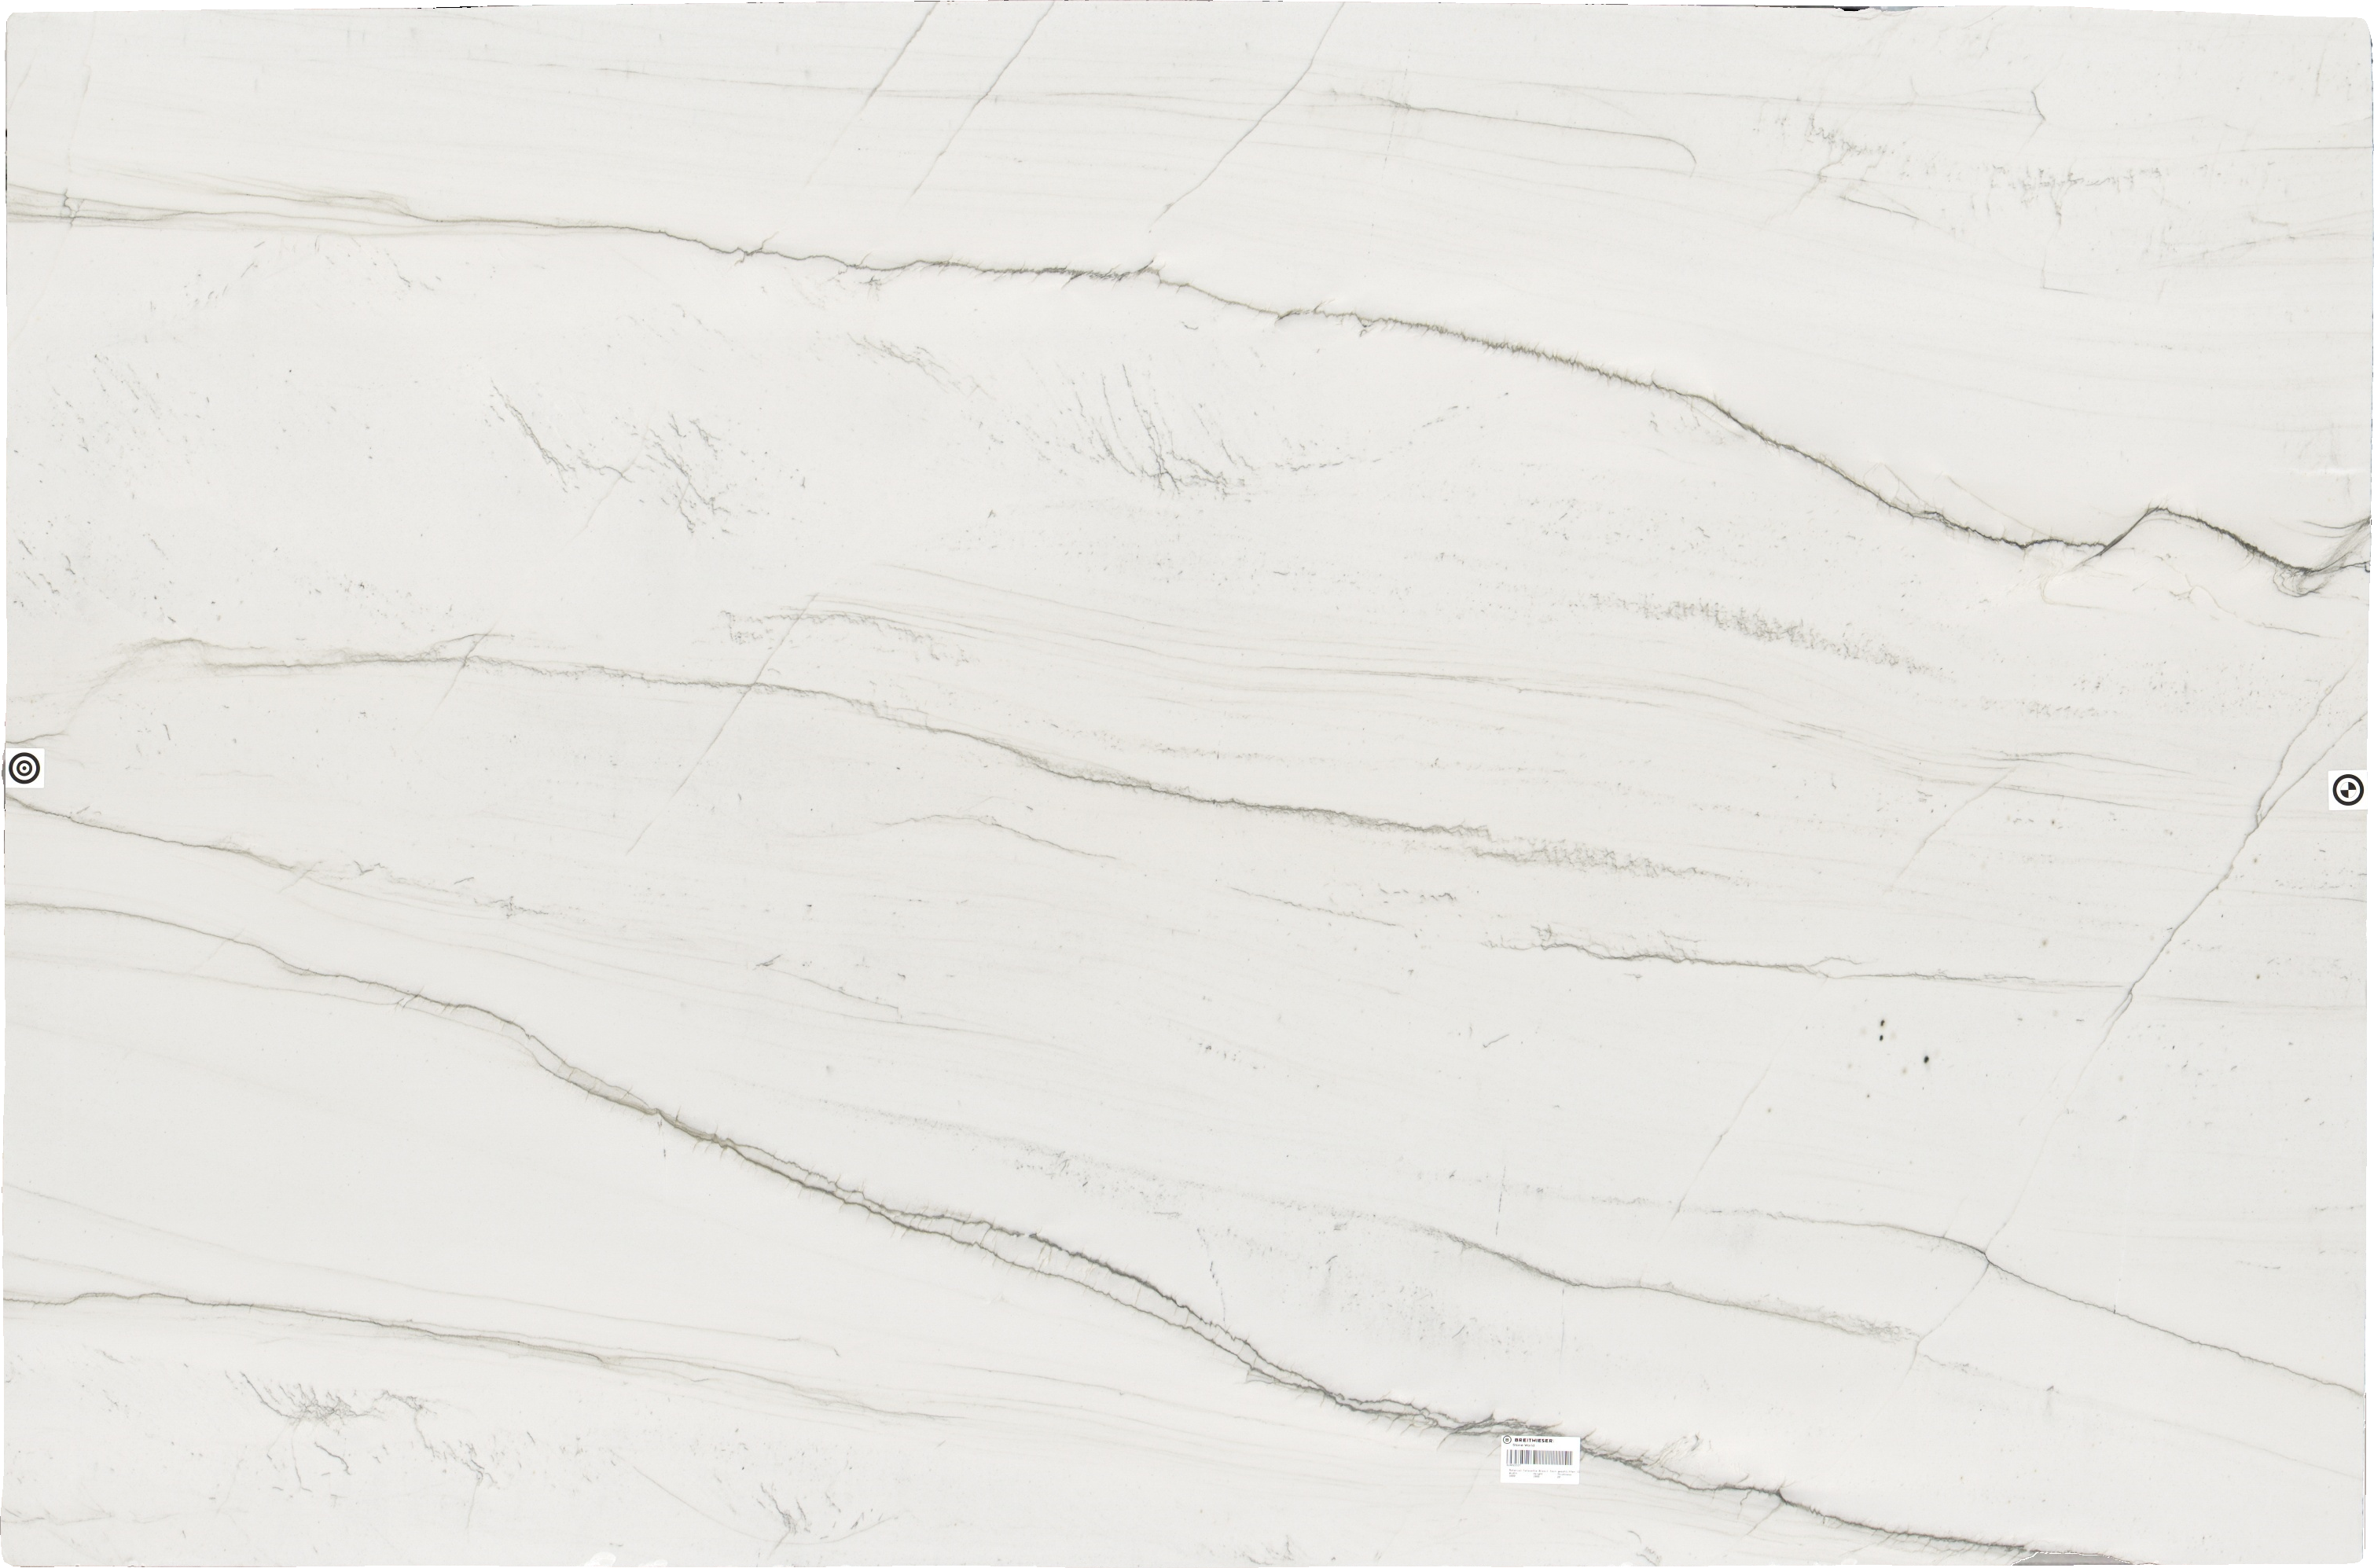
\includegraphics[width=.7\textwidth]{slabs/canny/canny_origin}
        \caption{HED}\label{fig:hed_compare}
    \end{figure}
    In figure~\ref*{fig:hed_compare} is possible to see the result of the HED algorithm.
\end{itemize}
\subsubsection{Milestone:}
At the end of the period the results showed that the best methods were the Meijering \& Contrast filter and the Canny Edge Detection.
HED was discarded because it was too slow and the results were not better than the other methods, many times it generates a lot of noise in the image (Random lines).
The two `winners' were able to extract the vein from the image, in an excellent way keeping in mind that was an unsupervised method.
\subsubsection{Improvements:}
One of the possible improvements is to use a supervised method to extract the vein.
This method will be more accurate than the non supervised method, because it will be trained to extract the vein.
But it requires a lot of time and hand labeled images to train the model.
\subsection{Fourth Period:}
This period was dedicated to the training of the network.
The network used was a pix2pix network, that is a network that uses a \gls{cgang} to generate images.
The training of the network was done using the dataset created in the previous periods and the hardware provided by the company. (See~\ref{subsec:hardware})
During this time different configuration of the network were tested, to find the best one, tweking the hyperparameters of the network.
The exact configuration of the network will be explained in chapter~\ref{cap:design-coding}.
\subsubsection{Milestone:}
At the end of the period the network was able to generate images of slabs, with a good variance of colors and textures (See~\ref*{fig:gen-images}).
%list of img generated
\begin{figure}
    \centering
    \includegraphics[width=.7\textwidth]{slabs/generated/amogus}
    \\
    \includegraphics[width=.7\textwidth]{slabs/generated/breton}
    \\
    \includegraphics[width=.7\textwidth]{slabs/generated/slab}
    \caption{Generated images}\label{fig:gen-images}
\end{figure}